

\tikzset{every picture/.style={line width=0.75pt}} %set default line width to 0.75pt        

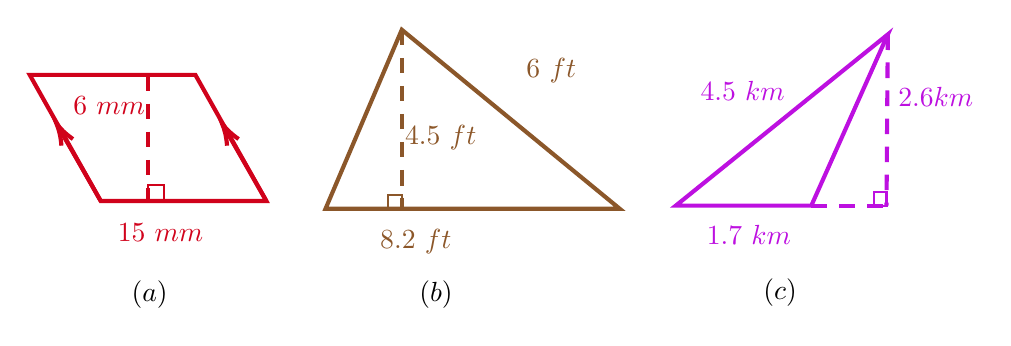
\begin{tikzpicture}[x=0.75pt,y=0.75pt,yscale=-1,xscale=1, scale=0.75]
%uncomment if require: \path (0,230); %set diagram left start at 0, and has height of 230

%Shape: Parallelogram [id:dp4045973963325873] 
\draw  [color={rgb, 255:red, 208; green, 2; blue, 27 }  ,draw opacity=1 ][line width=1.5]  (147.4,59) -- (41,59) -- (86.6,140) -- (193,140) -- cycle ;
%Straight Lines [id:da9796665582380797] 
\draw [color={rgb, 255:red, 208; green, 2; blue, 27 }  ,draw opacity=1 ][line width=1.5]  [dash pattern={on 5.63pt off 4.5pt}]  (117,59.5) -- (117,139.5) ;


%Shape: Square [id:dp06920862972284914] 
\draw  [color={rgb, 255:red, 208; green, 2; blue, 27 }  ,draw opacity=1 ] (117,129.5) -- (127,129.5) -- (127,139.5) -- (117,139.5) -- cycle ;
%Shape: Triangle [id:dp08961522547508038] 
\draw  [color={rgb, 255:red, 139; green, 87; blue, 42 }  ,draw opacity=1 ][line width=1.5]  (280,30) -- (420,145) -- (231,145) -- cycle ;
%Straight Lines [id:da8427678719260143] 
\draw [color={rgb, 255:red, 139; green, 87; blue, 42 }  ,draw opacity=1 ][line width=1.5]  [dash pattern={on 5.63pt off 4.5pt}]  (280,30) -- (280,145) ;


%Shape: Square [id:dp08529804115971995] 
\draw  [color={rgb, 255:red, 139; green, 87; blue, 42 }  ,draw opacity=1 ] (271,136) -- (280,136) -- (280,145) -- (271,145) -- cycle ;
%Shape: Polygon [id:ds9967185060442834] 
\draw  [color={rgb, 255:red, 189; green, 16; blue, 224 }  ,draw opacity=1 ][line width=1.5]  (456,143) -- (543.08,143) -- (592.22,33) -- cycle ;
%Straight Lines [id:da1558061082869422] 
\draw [color={rgb, 255:red, 189; green, 16; blue, 224 }  ,draw opacity=1 ][line width=1.5]  [dash pattern={on 5.63pt off 4.5pt}]  (592.22,33) -- (591.36,143) ;


%Straight Lines [id:da7378491629676467] 
\draw [color={rgb, 255:red, 189; green, 16; blue, 224 }  ,draw opacity=1 ][line width=1.5]  [dash pattern={on 5.63pt off 4.5pt}]  (543.08,143) -- (591.36,143) ;


%Shape: Rectangle [id:dp5477304566759069] 
\draw  [color={rgb, 255:red, 189; green, 16; blue, 224 }  ,draw opacity=1 ] (591.36,134) -- (583.6,134) -- (583.6,143) -- (591.36,143) -- cycle ;
%Straight Lines [id:da6859428859669638] 
\draw [color={rgb, 255:red, 208; green, 2; blue, 27 }  ,draw opacity=1 ][line width=1.5]    (86.6,140) -- (59.49,92.6) ;
\draw [shift={(58,90)}, rotate = 420.23] [color={rgb, 255:red, 208; green, 2; blue, 27 }  ,draw opacity=1 ][line width=1.5]    (14.21,-4.28) .. controls (9.04,-1.82) and (4.3,-0.39) .. (0,0) .. controls (4.3,0.39) and (9.04,1.82) .. (14.21,4.28)   ;

%Straight Lines [id:da26032096428140505] 
\draw [color={rgb, 255:red, 208; green, 2; blue, 27 }  ,draw opacity=1 ][line width=1.5]    (193,140) -- (165.89,92.6) ;
\draw [shift={(164.4,90)}, rotate = 420.23] [color={rgb, 255:red, 208; green, 2; blue, 27 }  ,draw opacity=1 ][line width=1.5]    (14.21,-4.28) .. controls (9.04,-1.82) and (4.3,-0.39) .. (0,0) .. controls (4.3,0.39) and (9.04,1.82) .. (14.21,4.28)   ;


% Text Node
\draw (92,79) node   {$\textcolor[rgb]{0.82,0.01,0.11}{6\ \text{mm}}$};
% Text Node
\draw (125,160) node   {$\textcolor[rgb]{0.82,0.01,0.11}{15\ }\textcolor[rgb]{0.82,0.01,0.11}{\text{mm}}$};
% Text Node
\draw (118,200) node   {$( a)$};
% Text Node
\draw (289,166) node   {$\textcolor[rgb]{0.55,0.34,0.16}{8.2\ \text{ ft}}$};
% Text Node
\draw (305,99) node   {$\textcolor[rgb]{0.55,0.34,0.16}{4.5\ \text{ft}}$};
% Text Node
\draw (376,56) node [color={rgb, 255:red, 139; green, 87; blue, 42 }  ,opacity=1 ]  {$6\ \text{ft}$};
% Text Node
\draw (302,200) node   {$( b)$};
% Text Node
\draw (503,162) node [color={rgb, 255:red, 189; green, 16; blue, 224 }  ,opacity=1 ]  {$1.7\ \text{km}$};
% Text Node
\draw (623,73) node [color={rgb, 255:red, 189; green, 16; blue, 224 }  ,opacity=1 ]  {$2.6\text{ km}$};
% Text Node
\draw (499,69) node [color={rgb, 255:red, 189; green, 16; blue, 224 }  ,opacity=1 ]  {$4.5\ \text{km}$};
% Text Node
\draw (523,199) node   {$( c)$};


\end{tikzpicture}